\documentclass[journal]{IEEEtran}

\usepackage[T1]{fontenc}
\usepackage{cite}
\usepackage{amsmath,amssymb}
\usepackage{graphicx}
\usepackage{booktabs}
\usepackage{multirow}
\usepackage{array}
\usepackage[per-mode=symbol,detect-all]{siunitx}
\usepackage{tikz}
\usetikzlibrary{arrows.meta,positioning,fit}
\usepackage{xurl}
\usepackage[hidelinks]{hyperref}

\sisetup{range-phrase=--,range-units=single}
\graphicspath{{figures/}}
% Auto-generated by paper/make_paper_assets.py - do not edit by hand.

\newcommand{\YieldL}{1608}
\newcommand{\PRL}{0.819}
\newcommand{\CUFL}{18.35}
\newcommand{\POAL}{1963}
\newcommand{\TdayL}{39.5}
\newcommand{\TmaxL}{57.3}
\newcommand{\TriseL}{10.1}
\newcommand{\RHL}{74.0}
\newcommand{\DewL}{1{,}163}
\newcommand{\SRL}{0.965}
\newcommand{\DegBaseL}{0.30}
\newcommand{\DegTHL}{0.34}
\newcommand{\DegPIDL}{0.15}
\newcommand{\DegCorrL}{0.09}
\newcommand{\DegTotL}{0.88}
\newcommand{\TOWL}{3{,}055}
\newcommand{\RHencL}{63.5}
\newcommand{\LifeL}{36{,}233}
\newcommand{\CapL}{80.9}
\newcommand{\LCOEL}{2.83}
\newcommand{\LossIncidenceAngleL}{3.44}
\newcommand{\LossSpectralL}{-0.23}
\newcommand{\LossSoilingL}{3.67}
\newcommand{\LossDewCondensationL}{0.02}
\newcommand{\LossModuleTemperatureL}{6.12}
\newcommand{\LossDcWiringMismatchMotionLidL}{3.46}
\newcommand{\LossInverterAndClippingL}{2.03}
\newcommand{\LossAvailabilityL}{1.00}
\newcommand{\YieldF}{1634}
\newcommand{\PRF}{0.837}
\newcommand{\CUFF}{18.66}
\newcommand{\POAF}{1953}
\newcommand{\TdayF}{36.5}
\newcommand{\TmaxF}{50.0}
\newcommand{\TriseF}{7.3}
\newcommand{\RHF}{77.5}
\newcommand{\DewF}{1{,}092}
\newcommand{\SRF}{0.988}
\newcommand{\DegBaseF}{0.30}
\newcommand{\DegTHF}{0.34}
\newcommand{\DegPIDF}{0.15}
\newcommand{\DegCorrF}{0.05}
\newcommand{\DegTotF}{0.84}
\newcommand{\TOWF}{3{,}719}
\newcommand{\RHencF}{68.4}
\newcommand{\LifeF}{37{,}004}
\newcommand{\CapF}{81.7}
\newcommand{\LCOEF}{3.54}
\newcommand{\LossIncidenceAngleF}{3.47}
\newcommand{\LossSpectralF}{-0.24}
\newcommand{\LossSoilingF}{1.27}
\newcommand{\LossDewCondensationF}{0.04}
\newcommand{\LossModuleTemperatureF}{4.78}
\newcommand{\LossDcWiringMismatchMotionLidF}{4.62}
\newcommand{\LossInverterAndClippingF}{2.03}
\newcommand{\LossAvailabilityF}{1.50}
\newcommand{\YieldS}{1590}
\newcommand{\PRS}{0.814}
\newcommand{\CUFS}{18.15}
\newcommand{\POAS}{1953}
\newcommand{\TdayS}{36.2}
\newcommand{\TmaxS}{49.4}
\newcommand{\TriseS}{7.0}
\newcommand{\RHS}{79.7}
\newcommand{\DewS}{1{,}389}
\newcommand{\SRS}{0.969}
\newcommand{\DegBaseS}{0.30}
\newcommand{\DegTHS}{0.36}
\newcommand{\DegPIDS}{0.21}
\newcommand{\DegCorrS}{0.30}
\newcommand{\DegTotS}{1.16}
\newcommand{\TOWS}{4{,}288}
\newcommand{\RHencS}{70.4}
\newcommand{\LifeS}{34{,}677}
\newcommand{\CapS}{75.5}
\newcommand{\LCOES}{4.43}
\newcommand{\LossIncidenceAngleS}{3.47}
\newcommand{\LossSpectralS}{-0.25}
\newcommand{\LossSoilingS}{3.29}
\newcommand{\LossDewCondensationS}{0.05}
\newcommand{\LossModuleTemperatureS}{4.64}
\newcommand{\LossDcWiringMismatchMotionLidS}{4.91}
\newcommand{\LossInverterAndClippingS}{2.03}
\newcommand{\LossAvailabilityS}{2.00}
\newcommand{\YieldLM}{1608}
\newcommand{\PRLM}{0.819}
\newcommand{\CUFLM}{18.35}
\newcommand{\POALM}{1963}
\newcommand{\TdayLM}{39.5}
\newcommand{\TmaxLM}{57.3}
\newcommand{\TriseLM}{10.1}
\newcommand{\RHLM}{74.0}
\newcommand{\DewLM}{1{,}163}
\newcommand{\SRLM}{0.965}
\newcommand{\DegBaseLM}{0.30}
\newcommand{\DegTHLM}{0.34}
\newcommand{\DegPIDLM}{0.02}
\newcommand{\DegCorrLM}{0.04}
\newcommand{\DegTotLM}{0.70}
\newcommand{\TOWLM}{3{,}055}
\newcommand{\RHencLM}{63.5}
\newcommand{\LifeLM}{37{,}002}
\newcommand{\CapLM}{84.5}
\newcommand{\LCOELM}{2.90}
\newcommand{\LossIncidenceAngleLM}{3.44}
\newcommand{\LossSpectralLM}{-0.23}
\newcommand{\LossSoilingLM}{3.67}
\newcommand{\LossDewCondensationLM}{0.02}
\newcommand{\LossModuleTemperatureLM}{6.12}
\newcommand{\LossDcWiringMismatchMotionLidLM}{3.46}
\newcommand{\LossInverterAndClippingLM}{2.03}
\newcommand{\LossAvailabilityLM}{1.00}
\newcommand{\YieldFM}{1634}
\newcommand{\PRFM}{0.837}
\newcommand{\CUFFM}{18.66}
\newcommand{\POAFM}{1953}
\newcommand{\TdayFM}{36.5}
\newcommand{\TmaxFM}{50.0}
\newcommand{\TriseFM}{7.3}
\newcommand{\RHFM}{77.5}
\newcommand{\DewFM}{1{,}092}
\newcommand{\SRFM}{0.988}
\newcommand{\DegBaseFM}{0.30}
\newcommand{\DegTHFM}{0.34}
\newcommand{\DegPIDFM}{0.01}
\newcommand{\DegCorrFM}{0.03}
\newcommand{\DegTotFM}{0.68}
\newcommand{\TOWFM}{3{,}719}
\newcommand{\RHencFM}{68.4}
\newcommand{\LifeFM}{37{,}698}
\newcommand{\CapFM}{84.9}
\newcommand{\LCOEFM}{3.60}
\newcommand{\LossIncidenceAngleFM}{3.47}
\newcommand{\LossSpectralFM}{-0.24}
\newcommand{\LossSoilingFM}{1.27}
\newcommand{\LossDewCondensationFM}{0.04}
\newcommand{\LossModuleTemperatureFM}{4.78}
\newcommand{\LossDcWiringMismatchMotionLidFM}{4.62}
\newcommand{\LossInverterAndClippingFM}{2.03}
\newcommand{\LossAvailabilityFM}{1.50}
\newcommand{\YieldSM}{1590}
\newcommand{\PRSM}{0.814}
\newcommand{\CUFSM}{18.15}
\newcommand{\POASM}{1953}
\newcommand{\TdaySM}{36.2}
\newcommand{\TmaxSM}{49.4}
\newcommand{\TriseSM}{7.0}
\newcommand{\RHSM}{79.7}
\newcommand{\DewSM}{1{,}389}
\newcommand{\SRSM}{0.969}
\newcommand{\DegBaseSM}{0.30}
\newcommand{\DegTHSM}{0.36}
\newcommand{\DegPIDSM}{0.02}
\newcommand{\DegCorrSM}{0.15}
\newcommand{\DegTotSM}{0.83}
\newcommand{\TOWSM}{4{,}288}
\newcommand{\RHencSM}{70.4}
\newcommand{\LifeSM}{36{,}045}
\newcommand{\CapSM}{81.9}
\newcommand{\LCOESM}{4.43}
\newcommand{\LossIncidenceAngleSM}{3.47}
\newcommand{\LossSpectralSM}{-0.25}
\newcommand{\LossSoilingSM}{3.29}
\newcommand{\LossDewCondensationSM}{0.05}
\newcommand{\LossModuleTemperatureSM}{4.64}
\newcommand{\LossDcWiringMismatchMotionLidSM}{4.91}
\newcommand{\LossInverterAndClippingSM}{2.03}
\newcommand{\LossAvailabilitySM}{2.00}
\newcommand{\GainYieldF}{1.6}
\newcommand{\GainYieldS}{-1.1}
\newcommand{\GainLifeF}{2.1}
\newcommand{\GainLifeS}{-4.3}
\newcommand{\GainLifeSM}{3.9}
\newcommand{\dTdayF}{3.0}
\newcommand{\dTmaxF}{7.3}
\newcommand{\WaterSaved}{11{,}700}
\newcommand{\GHI}{1{,}889}
\newcommand{\Tair}{28.1}
\newcommand{\RHair}{74.0}
\newcommand{\Rain}{1{,}043}
\newcommand{\SensLifeMin}{32{,}498}
\newcommand{\SensLifeMax}{37{,}005}
\newcommand{\SensDegMin}{0.78}
\newcommand{\SensDegMax}{1.49}
\newcommand{\SensSaltSpan}{2{,}854}
\newcommand{\SensMoistSpan}{1{,}674}
\newcommand{\SensDegPerK}{0.167}
\newcommand{\SensTOWZero}{2{,}253}
\newcommand{\SensTOWMax}{5{,}547}
\newcommand{\SensYieldLoPct}{4.6}
\newcommand{\BreakEvenSalinity}{$<$0.25}
\newcommand{\NSeeds}{20}
\newcommand{\EnsYieldF}{1.71}
\newcommand{\EnsYieldSdF}{0.08}
\newcommand{\EnsLifeF}{2.17}
\newcommand{\EnsLifeSdF}{0.10}
\newcommand{\EnsDegF}{-0.039}
\newcommand{\EnsDegSdF}{0.003}
\newcommand{\EnsYieldS}{-1.08}
\newcommand{\EnsYieldSdS}{0.05}
\newcommand{\EnsLifeS}{-4.32}
\newcommand{\EnsLifeSdS}{0.06}
\newcommand{\EnsDegS}{+0.288}
\newcommand{\EnsDegSdS}{0.002}
\newcommand{\EnsYieldLandMin}{1{,}570}
\newcommand{\EnsYieldLandMax}{1{,}649}
\newcommand{\EnsFreshWins}{20}


\newcommand{\RHs}{\mathit{RH}_{\mathrm{s}}}
\newcommand{\RHe}{\mathit{RH}_{\mathrm{e}}}
\newcommand{\TOWsym}{\mathit{TOW}}

\begin{document}

\title{Performance Analysis of Floating Solar Photovoltaic Systems for Humid and Saline Conditions:\\
A Coupled Thermal, Soiling and Degradation Assessment}

\author{Subrahmanyam~Tanala%
\thanks{Manuscript prepared October 2026.}%
\thanks{S. Tanala is with the Department of Electrical and Electronics Engineering, Anil Neerukonda Institute of Technology and Sciences (ANITS), Visakhapatnam 531162, Andhra Pradesh, India (e-mail: subrahmanyam.eee@anits.edu.in).}%
\thanks{The simulation code, input parameters and all scripts used to produce the results are openly available (see the Data Availability section).}}

\markboth{IEEE Transactions on Sustainable Energy}%
{Tanala: Performance Analysis of Floating PV for Humid and Saline Conditions}

\maketitle

\begin{abstract}
Floating photovoltaic (FPV) plants are usually credited with higher energy yield than land-based plants because the
water body cools the modules. In hot, humid, coastal regions the same water body also supplies moisture and, at
brackish or near-shore sites, airborne salt. Both accelerate soiling and degradation. This paper presents a coupled
hourly model that captures these competing effects. The model combines an over-water microclimate, a humidity-dependent
spectral correction, Faiman module temperature with dew formation, a dust and sea-salt soiling balance with NaCl
deliquescence, and a four-mechanism degradation model: intrinsic, Peck temperature--humidity with lagged encapsulant
moisture, potential-induced degradation (PID) with salt-assisted surface leakage, and chloride corrosion scaled by time
of wetness. Three 1-MWp plants at Visakhapatnam, India, are compared: coastal land-mounted, freshwater FPV and saline
FPV. Freshwater FPV runs \dTdayF~K cooler in daytime and yields \YieldF~kWh/kWp (+\GainYieldF\%) against
\YieldL~kWh/kWp on land. Saline FPV loses this advantage in the first year (\GainYieldS\%). Over 25 years the humid
air over water cancels the Arrhenius benefit of cooler modules for temperature--humidity degradation. At the saline site,
corrosion and PID raise total degradation to \DegTotS\%/yr against \DegTotL\%/yr on land, so lifetime energy falls by
\GainLifeS\%. PID-resistant, IEC~61701-certified modules recover \GainLifeSM\% of lifetime energy. The results hold over
\NSeeds{} independent weather realizations and are most sensitive to the salt load.
\end{abstract}

\begin{IEEEkeywords}
Floating photovoltaics, humidity, salinity, soiling, potential-induced degradation, corrosion, module temperature,
energy yield, degradation rate, levelized cost of energy.
\end{IEEEkeywords}

\section*{Nomenclature}
\addcontentsline{toc}{section}{Nomenclature}
\begin{IEEEdescription}[\IEEEusemathlabelsep\IEEEsetlabelwidth{$T_a, T_d, T_m$}]
\item[$G$] Plane-of-array (POA) irradiance (\si{\watt\per\square\metre}).
\item[$T_a, T_d, T_m$] Air, dew-point and module temperature (\si{\celsius}).
\item[$v$] Wind speed (\si{\metre\per\second}).
\item[$U_0, U_1$] Faiman heat-loss coefficients.
\item[$\RHs, \RHe$] Module-surface and encapsulant relative humidity (\%).
\item[$m_d, m_s$] Dust and salt surface density (\si{\gram\per\square\metre}).
\item[$\mathit{SR}$] Soiling ratio.
\item[$\TOWsym$] Time of wetness (h/yr).
\item[$D_{\mathrm{Cl}}$] Chloride deposition rate (\si{\milli\gram\per\square\metre\per\day}).
\item[$R$] Annual power degradation rate (\%/yr).
\item[$E_a$] Activation energy (eV).
\item[$k_B$] Boltzmann constant (\SI{8.617e-5}{\electronvolt\per\kelvin}).
\item[PR] Performance ratio.
\end{IEEEdescription}

%==========================================================================
\section{Introduction}
\IEEEPARstart{F}{loating} photovoltaic (FPV) systems place PV arrays on pontoons over reservoirs, lakes, lagoons and
sheltered coastal waters. They avoid competition for land, reduce evaporation from water-supply reservoirs and can share
grid infrastructure with hydropower plants~\cite{worldbank2019,sahu2016,trapani2015,oliveirapinto2020}. India has a
large inventory of reservoirs, salt pans and backwaters along a coast with high irradiation. FPV is therefore attractive
there, but many candidate sites are hot, humid and exposed to marine aerosol.

The performance case for FPV usually rests on the cooling effect of the water. Field studies in tropical Singapore found
lower module temperatures and higher performance ratios for well-ventilated FPV designs than for a rooftop
reference~\cite{liu2018}. Comparative measurements in the Netherlands and Singapore showed that the effective heat-loss
coefficient of FPV depends strongly on how open the floating structure is~\cite{dorenkamper2021}. Simulation of offshore
systems likewise predicts higher yield than for land-based systems, mainly because the modules run
cooler~\cite{golroodbari2020}. Most of these assessments focus on first-year energy~\cite{choi2014}.

The cooling, however, comes with more humid air. Humidity and temperature together drive hydrolysis, delamination and
corrosion in PV modules. The Peck model describes this damage as an Arrhenius function of temperature multiplied by a
power of relative humidity~\cite{peck1986}, and moisture ingress through polymer backsheets takes hours to
days~\cite{kempe2006}. Combined-stressor lifetime models confirm that humidity is a first-order variable for outdoor
degradation~\cite{kaaya2019}. Potential-induced degradation (PID) is strongly accelerated by humidity and surface
conductivity~\cite{pingel2010,hacke2011,iec62804}. Field surveys report higher degradation rates in hot climates than in
temperate ones~\cite{jordan2013}; in India the hot and humid zones are among the worst affected~\cite{dubey2014}. At
saline sites, chloride deposition and long time of wetness define the atmospheric corrosivity class of the
site~\cite{iso9223}. Salt mist is a recognized qualification stress for PV modules~\cite{iec61701}. Sea-salt deposits
also add to soiling, which is a major loss in sunny climates~\cite{sarver2013,kimber2006}.

What is missing is an analysis that couples these mechanisms through the same microclimate. If the water body lowers
module temperature but raises humidity, the net effect on lifetime energy is not obvious. It also differs between
freshwater and saline sites. This paper addresses that gap with the following contributions:
\begin{enumerate}
\item A coupled hourly model chain in which one over-water microclimate drives module temperature, dew, spectral
response, soiling and four degradation mechanisms, so their trade-offs are resolved consistently.
\item A moisture formulation based on module-surface relative humidity with a first-order encapsulant lag. It captures
why cooler modules see more moisture, and it couples this to PID through salt-assisted surface leakage.
\item A quantitative comparison of coastal land PV, freshwater FPV and saline FPV for a representative hot--humid
Indian site. The comparison covers first-year losses, mechanism-resolved degradation, 25-year energy and levelized cost
of energy (LCOE), with and without PID- and salt-mist-resistant modules.
\item A humidity--salinity sensitivity map and a \NSeeds-realization weather ensemble that separate robust conclusions
from weather noise.
\end{enumerate}

The rest of the paper is organized as follows. Section~\ref{sec:site} describes the site and the scenarios.
Section~\ref{sec:model} presents the model. Section~\ref{sec:results} reports the results, Section~\ref{sec:discussion}
discusses implications and limitations, and Section~\ref{sec:conclusion} concludes.

%==========================================================================
\section{Site and Study Scenarios}\label{sec:site}

The reference site is Visakhapatnam (\ang{17.69}~N, \ang{83.22}~E) on the Bay of Bengal. Its climate is tropical,
with a hot pre-monsoon season (April--May), the south-west monsoon (June--September) and the north-east monsoon with
cyclonic activity (October--November). An hourly typical year was synthesized from monthly normals
(Section~\ref{sec:weather}). It has a global horizontal irradiation (GHI) of \GHI~\si{\kilo\watt\hour\per\square\metre},
a mean air temperature of \Tair~\si{\celsius}, a mean relative humidity of \RHair\% and \Rain~mm of rain
(Fig.~\ref{fig:climate}).

\begin{figure}[!t]
\centering
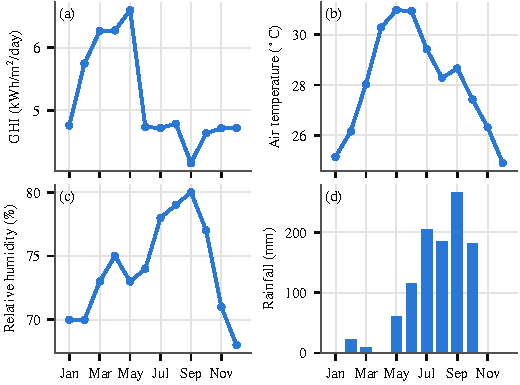
\includegraphics[width=\columnwidth]{climate.pdf}
\caption{Monthly climate of the synthetic Visakhapatnam typical year: (a) daily GHI, (b) air temperature, (c) relative
humidity and (d) rainfall.}
\label{fig:climate}
\end{figure}

Three 1-MWp (DC) plants with a DC/AC ratio of 1.2 and monocrystalline PERC modules
(\SI{-0.35}{\percent\per\kelvin}) are compared. Their parameters are listed in Table~\ref{tab:params}:
\begin{itemize}
\item \emph{Land PV}: a coastal ground-mounted plant on open racks with \ang{15} tilt (the reference).
\item \emph{FPV freshwater}: a pontoon plant with \ang{12} tilt on an inland reservoir with low chloride deposition.
\item \emph{FPV saline}: the same pontoon design on near-shore or brackish water (lagoon, salt pan or harbour) with high
salt and chloride loading.
\end{itemize}
Each plant is also simulated with PID-resistant modules certified to IEC~61701 severity level~6 (``mitigated'',~M).

\begin{table}[!t]
\caption{Scenario Parameters}
\label{tab:params}
\centering
\footnotesize
\setlength{\tabcolsep}{3.5pt}
\begin{tabular}{@{}lccc@{}}
\toprule
Parameter & Land & FPV fresh & FPV saline \\
\midrule
Tilt (\si{\degree}) & 15 & 12 & 12 \\
Albedo & 0.20 & 0.07 & 0.07 \\
$U_0$ (\si{\watt\per\square\metre\per\kelvin}) & 25.0 & 35.0 & 35.0 \\
$U_1$ (\si{\watt\second\per\cubic\metre\per\kelvin}) & 6.84 & 8.0 & 8.0 \\
Air--water coupling $\alpha$ & 0 & 0.25 & 0.30 \\
Dew-point rise $\Delta T_d$ (K) & 0 & 1.0 & 1.5 \\
Wind factor $k_v$ & 1.00 & 1.15 & 1.25 \\
Dust deposition (\si{\gram\per\square\metre\per\day}) & 0.15 & 0.04 & 0.03 \\
Salt deposition (\si{\gram\per\square\metre\per\day}) & 0.015 & 0.010 & 0.060 \\
$D_{\mathrm{Cl}}$ (\si{\milli\gram\per\square\metre\per\day}) & 30 & 8 & 180 \\
Wiring loss (\%) & 1.5 & 2.0 & 2.0 \\
Wave-motion mismatch (\%) & 0 & 0.7 & 1.0 \\
Availability (\%) & 99.0 & 98.5 & 98.0 \\
CAPEX (INR/Wp) & 35 & 45 & 52 \\
O\&M (INR/kWp/yr) & 450 & 550 & 750 \\
\bottomrule
\end{tabular}
\end{table}

%==========================================================================
\section{Modeling Framework}\label{sec:model}

The model chain is shown in Fig.~\ref{fig:chain}. All sub-models run at hourly resolution over one year. Degradation
rates are computed from the hourly stresses and then projected over the 25-year life of the plant. The established
irradiance and electrical models follow their reference formulations, as implemented, for example, in
pvlib~\cite{holmgren2018}.

\begin{figure}[!t]
\centering
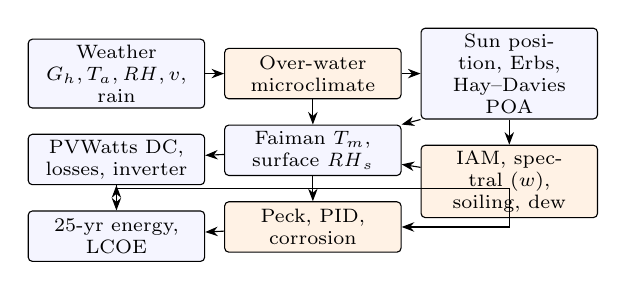
\begin{tikzpicture}[
  font=\scriptsize, node distance=3.2mm and 2.4mm,
  box/.style={draw, rounded corners=1.5pt, align=center, minimum height=6.4mm, inner sep=2pt, text width=21mm,
              fill=blue!4},
  hum/.style={box, fill=orange!10},
  arr/.style={-{Stealth[length=1.6mm]}, thin}]
\node[box] (wx) {Weather\\$G_h, T_a, \mathit{RH}, v$, rain};
\node[hum, right=of wx] (mc) {Over-water\\microclimate};
\node[box, right=of mc] (poa) {Sun position, Erbs,\\Hay--Davies POA};
\node[hum, below=of poa] (opt) {IAM, spectral ($w$),\\soiling, dew};
\node[box, below=of mc] (th) {Faiman $T_m$,\\surface $\mathit{RH}_s$};
\node[box, below=of wx] (el) {PVWatts DC,\\losses, inverter};
\node[hum, below=of th] (deg) {Peck, PID,\\corrosion};
\node[box, below=of el] (life) {25-yr energy,\\LCOE};
\draw[arr] (wx) -- (mc);
\draw[arr] (mc) -- (poa);
\draw[arr] (poa) -- (opt);
\draw[arr] (mc) -- (th);
\draw[arr] (poa.south west) -- (th.north east);
\draw[arr] (opt) -- (th);
\draw[arr] (th) -- (el);
\draw[arr] (opt.south) |- ([yshift=-1.6mm]th.south) -| (el.south);
\draw[arr] (th) -- (deg);
\draw[arr] (opt.south) |- (deg.east);
\draw[arr] (el) -- (life);
\draw[arr] (deg) -- (life);
\end{tikzpicture}
\caption{Coupled model chain. Shaded blocks carry an explicit dependence on humidity or salinity.}
\label{fig:chain}
\end{figure}

\subsection{Weather and Over-Water Microclimate}\label{sec:weather}
The synthetic year draws daily rain occurrence and amounts, a first-order autoregressive daily clearness index and
daily temperature anomalies from monthly normals. Hourly GHI is the Haurwitz clear-sky value~\cite{haurwitz1945} scaled
by the clearness index. Air temperature follows an asymmetric diurnal cycle, with the minimum near 05:00 and the maximum
near 14:00. Holding the dew point $T_d$ constant over each day reproduces the observed diurnal swing in relative
humidity. Wind speed includes an afternoon sea breeze. Measured series can be used in place of the synthetic year.

Over water, the air temperature is pulled towards the water temperature $T_w$, taken as the 30-day running mean of air
temperature plus \SI{0.5}{\kelvin}. The dew point rises by $\Delta T_d$ because of evaporation, and the wind speed
increases over the smoother surface:
\begin{equation}
\begin{gathered}
T_a' = T_a + \alpha\,(T_w - T_a),\qquad v' = k_v v,\\
T_d' = \min(T_d + \Delta T_d,\,T_a').
\end{gathered}
\label{eq:micro}
\end{equation}
Relative humidity follows from the Magnus relation $e_s(T)=6.112\exp[17.62T/(243.12+T)]$~hPa as
$\mathit{RH}=100\,e_s(T_d')/e_s(T_a')$.

\subsection{Irradiance, Incidence and Spectrum}
Solar position uses Spencer's series~\cite{spencer1971}. GHI is decomposed with the Erbs
correlation~\cite{erbs1982} and transposed to the array plane with the Hay--Davies model~\cite{hay1980}:
\begin{multline}
G = G_b\cos\theta + G_d\left[A_i R_b + (1-A_i)\tfrac{1+\cos\beta}{2}\right]\\
+ \rho\,G_h\tfrac{1-\cos\beta}{2},
\label{eq:poa}
\end{multline}
where $\theta$ is the angle of incidence, $\beta$ the tilt, $A_i$ the anisotropy index, $R_b$ the beam ratio and
$\rho$ the albedo. Water has a much lower albedo than land (0.07 against 0.20). Beam reflection losses use the ASHRAE
modifier $\mathrm{IAM}=1-b_0(1/\cos\theta-1)$ with $b_0=0.05$; diffuse and ground-reflected light take a constant
factor of 0.95.

Humid air absorbs mainly in infrared bands where crystalline silicon responds weakly. The spectral mismatch factor for
mono-Si is therefore computed from the Kasten--Young air mass $\mathit{AM}$~\cite{kasten1989} and the precipitable
water $w$ (cm), estimated from surface temperature and humidity~\cite{gueymard1994}:
\begin{equation}
M = c_1 + c_2\mathit{AM} + c_3 w + c_4\sqrt{\mathit{AM}} + c_5\sqrt{w} + c_6\,\mathit{AM}/\sqrt{w},
\label{eq:spectral}
\end{equation}
with the mono-Si coefficients of~\cite{lee2016}.

\subsection{Module Temperature, Surface Humidity and Dew}
Module temperature follows the Faiman model~\cite{faiman2008}. A net long-wave loss of
$q_{\mathrm{sky}}=\SI{40}{\watt\per\square\metre}$ to the night sky applies when $G<\SI{50}{\watt\per\square\metre}$:
\begin{equation}
T_m = T_a' + \frac{G - q_{\mathrm{sky}}\,\mathbb{1}[G<50]}{U_0 + U_1 v'}.
\label{eq:faiman}
\end{equation}
The land coefficients are the open-rack defaults. The FPV values lie within the range of heat-loss coefficients
reported for pontoon systems~\cite{liu2018,dorenkamper2021}. The relative humidity of the air layer in contact with the
glass is
\begin{equation}
\RHs = 100\,e_s(T_d')/e_s(T_m),
\label{eq:rhs}
\end{equation}
so a hot module is effectively dry and a module colder than the dew point is wet. Dew forms when
$T_m - T_d' < \SI{1}{\kelvin}$ and persists after sunrise until $T_m - T_d' > \SI{4}{\kelvin}$. While dew is present, a
4\% optical loss applies.

\subsection{Dust and Sea-Salt Soiling}
Dust and salt surface densities evolve by a daily mass balance. Dust accumulates at $r_d$, and salt at $r_s\,v/v_0$ with
$v_0=\SI{3}{\metre\per\second}$, because sea-spray generation rises with wind. Rain above \SI{2}{mm/day} removes a
fraction $\eta_d f_\beta$ of the dust and $\eta_s f_\beta$ of the salt. Here $\eta_d = 0.80$, $\eta_s = 0.95$ (salt is
soluble) and $f_\beta=\sin\beta/\sin\ang{20}$, so cleaning is less effective at low tilt. When the daily maximum RH
exceeds the NaCl deliquescence point of 75\%, the dissolved salt recrystallizes as a crust that cements dust to the
glass. On such days the dust-cleaning efficiency is halved. All plants are cleaned every 15~days with 95\% efficiency.
The soiling ratio is
\begin{equation}
\mathit{SR} = \max\left(\mathit{SR}_{\min},\,1 - k_d m_d - k_s m_s\right),
\label{eq:soiling}
\end{equation}
with $k_d=0.035$ and $k_s=\SI{0.060}{\square\metre\per\gram}$.

\subsection{Electrical Model}
The effective irradiance $G_{\mathrm{eff}}$ includes the incidence, spectral, soiling and dew corrections. DC power
follows the PVWatts model~\cite{dobos2014}:
\begin{equation}
P_{\mathrm{dc}} = P_0\,\frac{G_{\mathrm{eff}}}{1000}\left[1+\gamma(T_m-25)\right]\prod_j(1-\ell_j),
\label{eq:pdc}
\end{equation}
where $\gamma=\SI{-0.0035}{\per\kelvin}$ and $\ell_j$ are the wiring, mismatch, wave-motion and light-induced
degradation (LID, 1\%) losses. The PVWatts inverter curve (nominal efficiency 98\%) applies, with clipping at the AC
rating, followed by the availability factor. Each loss is reported as a percentage of the energy at the preceding
stage of the chain.

\subsection{Degradation Model}
The annual degradation rate is the sum of four mechanisms:
\begin{equation}
R = R_0 + R_{\mathrm{TH}} + R_{\mathrm{PID}} + R_{\mathrm{C}}.
\label{eq:R}
\end{equation}
The intrinsic term $R_0=0.30$\%/yr covers ultraviolet exposure and thermal cycling and does not depend on the site.

\emph{Temperature--humidity.} Moisture inside the encapsulant follows the surface humidity with a first-order lag of time
constant $\tau=\SI{48}{h}$, representing diffusion through the backsheet~\cite{kempe2006}:
\begin{equation}
\RHe(t) = \RHe(t-1) + \kappa\,\bigl[\RHs(t)-\RHe(t-1)\bigr],
\label{eq:rhe}
\end{equation}
with $\kappa = 1-e^{-\Delta t/\tau}$. With the Arrhenius factor
\begin{equation}
a_E(T_m) = \exp\!\left[-\frac{E}{k_B}\left(\frac{1}{T_m}-\frac{1}{T_{\mathrm{ref}}}\right)\right],
\label{eq:arr}
\end{equation}
the Peck rate~\cite{peck1986} is averaged over the year:
\begin{equation}
R_{\mathrm{TH}} = R_{\mathrm{TH}}^{\mathrm{ref}}\left\langle a_{E_a}(T_m)
\left(\frac{\RHe}{\mathit{RH}_{\mathrm{ref}}}\right)^{n}\right\rangle,
\label{eq:peck}
\end{equation}
with $E_a=\SI{0.79}{eV}$, $n=3$, $T_{\mathrm{ref}}=\SI{25}{\celsius}$ and $\mathit{RH}_{\mathrm{ref}}=60\%$. Because
$\RHs$ depends on $T_m$, cooling a module lowers the Arrhenius factor but raises $\RHe$; \eqref{eq:peck} resolves this
trade-off.

\emph{Potential-induced degradation.} PID acts only while the array is energized ($G>\SI{50}{\watt\per\square\metre}$).
Its rate depends on module temperature and on the probability that a conductive film covers the glass:
\begin{equation}
R_{\mathrm{PID}} = R_{\mathrm{PID}}^{\mathrm{ref}}(1-\mu_{\mathrm{PID}})
\bigl\langle a_{E_{\mathrm{PID}}}(T_m)\,f_{\mathrm{leak}}\bigr\rangle_{\mathrm{on}},
\label{eq:pid}
\end{equation}
\begin{equation}
f_{\mathrm{leak}} = \left[1+\exp\left(-\frac{\mathit{RH} - (\mathit{RH}_{50} - \Delta_s\,s)}{5}\right)\right]^{-1},
\label{eq:leak}
\end{equation}
where $E_{\mathrm{PID}}=\SI{0.9}{eV}$, $\mathit{RH}_{50}=70\%$, and $s=\min(m_s/0.5,1)$ is the salt coverage. A full
hygroscopic salt film lowers the threshold by $\Delta_s=15\%$~RH. The factor $\mu_{\mathrm{PID}}=0.9$ applies to
PID-resistant modules~\cite{pingel2010,hacke2011,iec62804}.

\emph{Chloride corrosion.} Following the ISO~9223 logic of time of wetness and chloride deposition~\cite{iso9223}, the
corrosion rate is
\begin{equation}
R_{\mathrm{C}} = R_{\mathrm{C}}^{\mathrm{ref}}\,\frac{\TOWsym}{\TOWsym_{\mathrm{ref}}}
\sqrt{\frac{D_{\mathrm{Cl}}}{D_{\mathrm{ref}}}}\,(1-\mu_{\mathrm{C}}),
\label{eq:corr}
\end{equation}
where $\TOWsym$ counts the hours with $\mathit{RH}>80\%$ or with dew on the module. The reference values are
$\TOWsym_{\mathrm{ref}}=\SI{2500}{h}$ and $D_{\mathrm{ref}}=\SI{60}{\milli\gram\per\square\metre\per\day}$, and
$\mu_{\mathrm{C}}=0.5$ for IEC~61701 severity-6 modules~\cite{iec61701}.

The reference rates ($R_{\mathrm{TH}}^{\mathrm{ref}}=0.10$, $R_{\mathrm{PID}}^{\mathrm{ref}}=0.06$ and
$R_{\mathrm{C}}^{\mathrm{ref}}=0.10$\%/yr) were calibrated so that standard modules on land at this site degrade by
roughly 1\%/yr. That is the order of magnitude reported for hot--humid Indian climates~\cite{dubey2014}, and above the
global median of about 0.5\%/yr~\cite{jordan2013}.

\subsection{Lifetime Energy and Economics}
Year-$y$ energy is $E_y = E_1(1-R/100)^{y-1}$ over a life of $N=25$ years. The LCOE is
\begin{equation}
\mathrm{LCOE} = \frac{C_0 + \sum_{y=1}^{N} O_y(1+r)^{-y}}{\sum_{y=1}^{N}E_y(1+r)^{-y}},
\label{eq:lcoe}
\end{equation}
with a discount rate $r=9\%$ and O\&M costs $O_y$ that escalate by 5\%/yr. The costs in Table~\ref{tab:params} are
illustrative Indian-market values. For the freshwater plant, the evaporation avoided by shading
(\SI{10}{\square\metre\per\kilo\watt p}, 65\% suppression of \SI{1800}{mm/yr} pan evaporation) is reported as a
co-benefit.

%==========================================================================
\section{Results}\label{sec:results}

\subsection{Thermal Behavior}
Fig.~\ref{fig:temp} shows the mean diurnal module temperature in May, the hottest month. Over the year, floating modules
run \dTdayF~K cooler in daytime than land-mounted modules, and their peak temperature is \dTmaxF~K lower
(Table~\ref{tab:perf}). The mean daytime module-to-air temperature rise falls from \TriseL~K on land to \TriseF~K
(freshwater) and \TriseS~K (saline). The saline plant runs slightly cooler still because of its stronger air--water
coupling and higher wind. At night the picture reverses. Modules on land radiate below the air temperature, while over
water the air stays warmer and the modules follow it; yet the higher dew point keeps floating modules closer to
condensation. Dew is present on the glass for \DewL~h on land, \DewF~h on freshwater and \DewS~h on saline water.

\begin{figure}[!t]
\centering
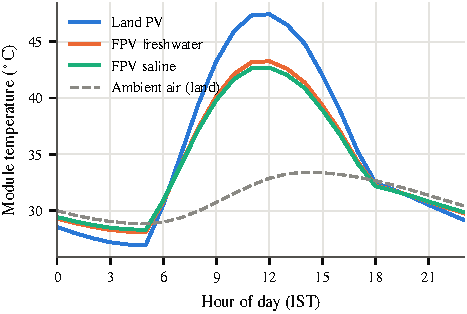
\includegraphics[width=\columnwidth]{module_temperature.pdf}
\caption{Mean module temperature by hour of day in May for the three plants, with the site air temperature.}
\label{fig:temp}
\end{figure}

\begin{table}[!t]
\caption{Year-1 Performance}
\label{tab:perf}
\centering
\footnotesize
\setlength{\tabcolsep}{3pt}
\begin{tabular}{@{}lccc@{}}
\toprule
Metric & Land & FPV fresh & FPV saline \\
\midrule
POA irradiation (\si{\kilo\watt\hour\per\square\metre}) & \POAL & \POAF & \POAS \\
Specific yield (kWh/kWp) & \YieldL & \textbf{\YieldF} & \YieldS \\
Performance ratio & \PRL & \textbf{\PRF} & \PRS \\
CUF, DC basis (\%) & \CUFL & \CUFF & \CUFS \\
Mean daytime $T_m$ (\si{\celsius}) & \TdayL & \TdayF & \TdayS \\
Maximum $T_m$ (\si{\celsius}) & \TmaxL & \TmaxF & \TmaxS \\
Mean $T_m - T_a$, daytime (K) & \TriseL & \TriseF & \TriseS \\
Mean air RH at array (\%) & \RHL & \RHF & \RHS \\
Dew on glass (h/yr) & \DewL & \DewF & \DewS \\
Mean daytime soiling ratio & \SRL & \SRF & \SRS \\
\bottomrule
\end{tabular}
\end{table}

\subsection{Energy Yield and Loss Breakdown}
Freshwater FPV gives the highest first-year specific yield, \YieldF~kWh/kWp, which is \GainYieldF\% above the land
plant. Its PR is \PRF{} against \PRL{} (Table~\ref{tab:perf}). The loss breakdown in Table~\ref{tab:loss} and
Fig.~\ref{fig:loss} shows where the gain comes from. The temperature loss falls from \LossModuleTemperatureL\% to
\LossModuleTemperatureF\%, and the soiling loss falls from \LossSoilingL\% to \LossSoilingF\% because little dust
reaches the water surface. Part of this gain is given back by DC losses (longer cable runs and wave-induced mismatch:
\LossDcWiringMismatchMotionLidF\% against \LossDcWiringMismatchMotionLidL\%), by lower availability and by
slightly lower POA irradiation from the lower tilt and the low albedo of water.

The saline plant has the same thermal advantage (\LossModuleTemperatureS\%). Salt soiling, however, brings its soiling
loss back to the land level (\LossSoilingS\%). With the highest DC and availability losses, its first-year yield is
\YieldS~kWh/kWp (\GainYieldS\% against land). Humidity itself has a small but beneficial spectral effect: precipitable
water shifts the spectrum towards wavelengths that c-Si converts well, which gives a gain of about
\SI{0.25}{\percent} at all three sites. Dew causes a loss of less than 0.1\% because condensate evaporates within the
first hours after sunrise.

\begin{table}[!t]
\caption{Year-1 Loss Breakdown (\% of Preceding Stage)}
\label{tab:loss}
\centering
\footnotesize
\begin{tabular}{@{}lccc@{}}
\toprule
Loss stage & Land & FPV fresh & FPV saline \\
\midrule
Incidence angle (IAM) & \LossIncidenceAngleL & \LossIncidenceAngleF & \LossIncidenceAngleS \\
Spectral (humidity) & \LossSpectralL & \LossSpectralF & \LossSpectralS \\
Soiling (dust + salt) & \LossSoilingL & \LossSoilingF & \LossSoilingS \\
Dew / condensation & \LossDewCondensationL & \LossDewCondensationF & \LossDewCondensationS \\
Module temperature & \LossModuleTemperatureL & \LossModuleTemperatureF & \LossModuleTemperatureS \\
DC (wiring, mismatch, motion, LID) & \LossDcWiringMismatchMotionLidL & \LossDcWiringMismatchMotionLidF & \LossDcWiringMismatchMotionLidS \\
Inverter and clipping & \LossInverterAndClippingL & \LossInverterAndClippingF & \LossInverterAndClippingS \\
Availability & \LossAvailabilityL & \LossAvailabilityF & \LossAvailabilityS \\
\bottomrule
\end{tabular}
\end{table}

\begin{figure}[!t]
\centering
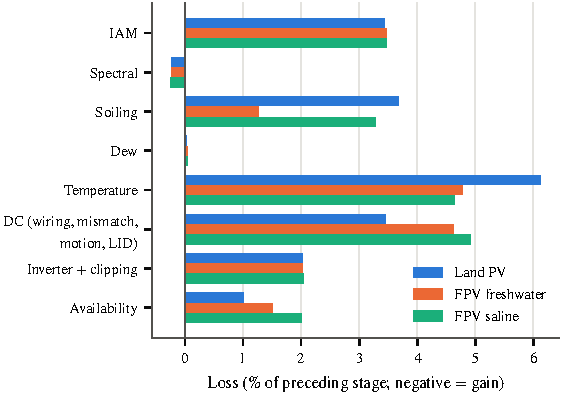
\includegraphics[width=\columnwidth]{losses.pdf}
\caption{Year-1 loss breakdown. Negative values are gains.}
\label{fig:loss}
\end{figure}

Fig.~\ref{fig:pr} shows the monthly PR. The FPV advantage is largest in the dry, clear months (November--May). In the
pre-monsoon months the saline plant performs worst: heavy salt deposition under the strong onshore wind meets a
lack of rain. During the monsoon frequent rain cleans all three arrays and the thermal advantage shrinks under cloudy
skies, so the gap narrows. Fig.~\ref{fig:soil} shows the daily soiling ratio. Between cleanings, salt deposition on the
saline plant produces a saw-tooth pattern similar to dust soiling on land, while the freshwater array stays close to
clean.

\begin{figure}[!t]
\centering
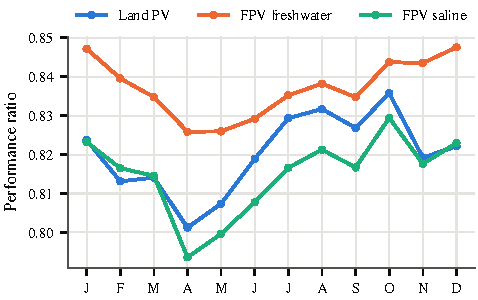
\includegraphics[width=\columnwidth]{monthly_pr.pdf}
\caption{Monthly performance ratio.}
\label{fig:pr}
\end{figure}

\begin{figure}[!t]
\centering
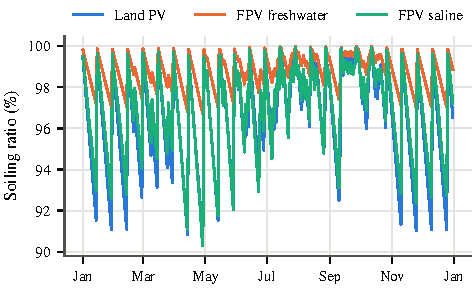
\includegraphics[width=\columnwidth]{soiling.pdf}
\caption{Daily soiling ratio with rain cleaning, NaCl deliquescence and 15-day manual cleaning.}
\label{fig:soil}
\end{figure}

\subsection{Degradation}
Table~\ref{tab:deg} and Fig.~\ref{fig:deg} resolve the degradation rate by mechanism. The central result is the
temperature--humidity term. Floating modules are cooler, but their encapsulant equilibrates at a higher moisture level:
mean $\RHe$ is \RHencL\% on land, \RHencF\% on freshwater and \RHencS\% on saline water. Through the cubic humidity
dependence of \eqref{eq:peck}, this cancels the Arrhenius benefit. $R_{\mathrm{TH}}$ is \DegTHL\%/yr on land,
\DegTHF\%/yr on freshwater and \DegTHS\%/yr on saline water. For hydrolysis-type damage, \emph{cooling by water does not
translate into slower ageing at a humid site}.

PID is slightly lower on freshwater (\DegPIDF\%/yr) than on land (\DegPIDL\%/yr), because the higher activation energy
rewards cooler modules. On saline water it is highest (\DegPIDS\%/yr), because the hygroscopic salt film makes the glass
conductive at lower RH. Corrosion separates the sites most clearly. The time of wetness grows from \TOWL~h/yr on land to
\TOWF~h/yr and \TOWS~h/yr over water. Combined with \SI{180}{\milli\gram\per\square\metre\per\day} of chloride
deposition, this gives $R_{\mathrm{C}}=\DegCorrS$\%/yr on saline water against \DegCorrL\%/yr on land and
\DegCorrF\%/yr on freshwater. In total, the freshwater plant degrades at \DegTotF\%/yr, close to the land plant
(\DegTotL\%/yr), while the saline plant degrades at \DegTotS\%/yr.

\begin{figure}[!t]
\centering
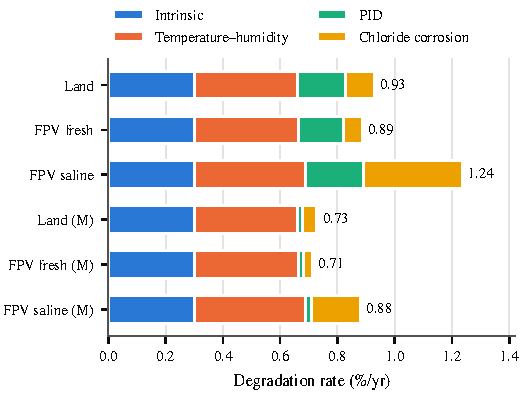
\includegraphics[width=\columnwidth]{degradation.pdf}
\caption{Annual degradation rate by mechanism. (M): PID-resistant, IEC~61701 severity-6 modules.}
\label{fig:deg}
\end{figure}

\begin{table*}[!t]
\caption{Degradation, Lifetime Energy and LCOE (per MWp; M = PID-Resistant, IEC 61701 Severity-6 Modules)}
\label{tab:deg}
\centering
\footnotesize
\begin{tabular}{@{}lcccccc@{}}
\toprule
 & Land & FPV fresh & FPV saline & Land (M) & FPV fresh (M) & FPV saline (M) \\
\midrule
$R_0$ intrinsic (\%/yr) & \DegBaseL & \DegBaseF & \DegBaseS & \DegBaseLM & \DegBaseFM & \DegBaseSM \\
$R_{\mathrm{TH}}$ temperature--humidity (\%/yr) & \DegTHL & \DegTHF & \DegTHS & \DegTHLM & \DegTHFM & \DegTHSM \\
$R_{\mathrm{PID}}$ (\%/yr) & \DegPIDL & \DegPIDF & \DegPIDS & \DegPIDLM & \DegPIDFM & \DegPIDSM \\
$R_{\mathrm{C}}$ chloride corrosion (\%/yr) & \DegCorrL & \DegCorrF & \DegCorrS & \DegCorrLM & \DegCorrFM & \DegCorrSM \\
\textbf{Total $R$ (\%/yr)} & \textbf{\DegTotL} & \textbf{\DegTotF} & \textbf{\DegTotS} & \textbf{\DegTotLM} & \textbf{\DegTotFM} & \textbf{\DegTotSM} \\
Time of wetness (h/yr) & \TOWL & \TOWF & \TOWS & \TOWLM & \TOWFM & \TOWSM \\
Mean encapsulant RH (\%) & \RHencL & \RHencF & \RHencS & \RHencLM & \RHencFM & \RHencSM \\
Capacity in year 25 (\%) & \CapL & \CapF & \CapS & \CapLM & \CapFM & \CapSM \\
25-year energy (MWh) & \LifeL & \textbf{\LifeF} & \LifeS & \LifeLM & \textbf{\LifeFM} & \LifeSM \\
LCOE (INR/kWh) & \LCOEL & \LCOEF & \LCOES & \LCOELM & \LCOEFM & \LCOESM \\
\bottomrule
\end{tabular}
\end{table*}

\subsection{Lifetime Energy, Mitigation and Cost}
Over 25 years (Fig.~\ref{fig:life}), freshwater FPV delivers \LifeF~MWh/MWp, \GainLifeF\% more than the land plant. The
saline plant delivers \LifeS~MWh/MWp, which is \GainLifeS\% less, and keeps only \CapS\% of its initial capacity in
year~25. PID-resistant, IEC~61701 severity-6 modules reduce the saline degradation rate to \DegTotSM\%/yr and raise its
lifetime energy by \GainLifeSM\%. Even so, the mitigated saline plant does not reach the unmitigated land plant. On land
and freshwater the same modules lower the rate to \DegTotLM\% and \DegTotFM\%/yr.

With the assumed costs, FPV is more expensive per kWh: \LCOEF~INR/kWh on freshwater and \LCOES~INR/kWh on saline water,
against \LCOEL~INR/kWh on land. The cost of the floats, mooring and marine-grade balance of system dominates over the
yield gain. For the saline plant, the mitigated modules (assumed to cost \SI{1.5}{INR/Wp} more) already lower the LCOE
from \LCOES{} to \LCOESM~INR/kWh. FPV is therefore justified mainly by land savings and, on freshwater, by
co-benefits: the freshwater plant avoids about \WaterSaved~\si{\cubic\metre} of reservoir evaporation per MWp each year.

\begin{figure}[!t]
\centering
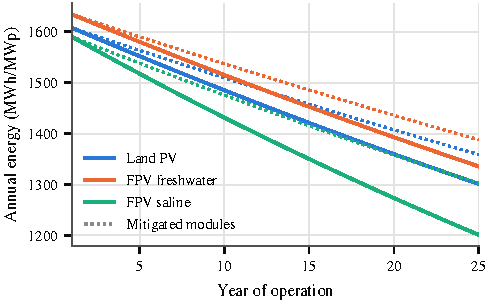
\includegraphics[width=\columnwidth]{lifetime.pdf}
\caption{Annual energy over 25 years of operation. Dotted lines: PID-resistant, IEC~61701 severity-6 modules.}
\label{fig:life}
\end{figure}

\subsection{Sensitivity to Humidity and Salinity}
For the saline plant, Fig.~\ref{fig:sens} varies the dew-point rise over water from 0 to \SI{2.5}{\kelvin} and scales
the salt and chloride deposition together from $0.25\times$ to $2\times$ the baseline. The degradation rate ranges from
\SensDegMin{} to \SensDegMax\%/yr, and 25-year energy ranges from \SensLifeMin{} to \SensLifeMax~MWh/MWp. Each kelvin of
extra dew point adds about \SensDegPerK\%/yr of degradation at baseline salinity, because the time of wetness grows from
\SensTOWZero{} to \SensTOWMax~h/yr across the sweep. Across the full ranges swept, salinity moves lifetime energy by
about \SensSaltSpan~MWh/MWp and moisture by about \SensMoistSpan~MWh/MWp. Salinity also cuts first-year yield by
\SensYieldLoPct\% between the lowest and highest salt loads, through soiling. At the baseline moisture level
(+\SI{1.5}{\kelvin}), the saline plant matches the lifetime energy of the land plant only if the salt load falls to
\BreakEvenSalinity$\times$ the baseline.

\begin{figure*}[!t]
\centering
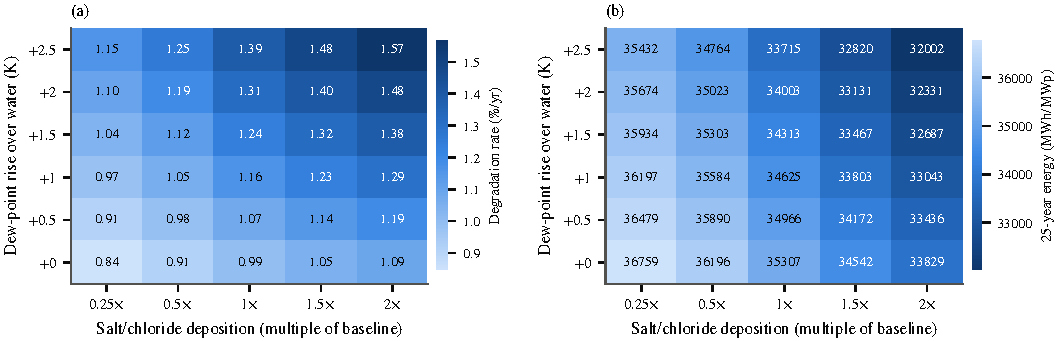
\includegraphics[width=\textwidth]{sensitivity.pdf}
\caption{Sensitivity of the saline FPV plant to the dew-point rise over water and the salt/chloride load: (a) total
degradation rate and (b) 25-year energy.}
\label{fig:sens}
\end{figure*}

\subsection{Robustness to Weather Variability}
To check that the conclusions do not depend on one synthetic year, the three plants were simulated for \NSeeds{}
independent weather realizations (Table~\ref{tab:ens}, Fig.~\ref{fig:ens}). The land yield varies between
\EnsYieldLandMin{} and \EnsYieldLandMax~kWh/kWp, but the differences between plants are stable. Freshwater FPV
outperforms land in \EnsFreshWins{} of \NSeeds{} years, and the standard deviations of the relative differences are below
0.1 percentage point. The ranking of the plants is the same in every realization.

\begin{table}[!t]
\caption{Differences From Land PV Over \NSeeds{} Weather Realizations (Mean $\pm$ SD)}
\label{tab:ens}
\centering
\footnotesize
\setlength{\tabcolsep}{4pt}
\begin{tabular}{@{}lcc@{}}
\toprule
 & FPV fresh & FPV saline \\
\midrule
Year-1 yield (\%) & $+\EnsYieldF \pm \EnsYieldSdF$ & $\EnsYieldS \pm \EnsYieldSdS$ \\
25-year energy (\%) & $+\EnsLifeF \pm \EnsLifeSdF$ & $\EnsLifeS \pm \EnsLifeSdS$ \\
Degradation rate (\%/yr) & $\EnsDegF \pm \EnsDegSdF$ & $\EnsDegS \pm \EnsDegSdS$ \\
\bottomrule
\end{tabular}
\end{table}

\begin{figure}[!t]
\centering
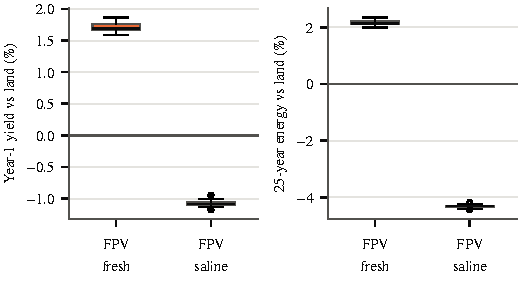
\includegraphics[width=\columnwidth]{ensemble.pdf}
\caption{Distribution over \NSeeds{} weather realizations of the year-1 yield and 25-year energy of the FPV plants
relative to land PV.}
\label{fig:ens}
\end{figure}

%==========================================================================
\section{Discussion}\label{sec:discussion}

\subsection{Implications for Design and Siting}
The results separate two questions that are often merged: whether FPV produces more energy in its first year, and whether
it produces more over its life. For freshwater reservoirs in a hot--humid climate both answers are yes, by \GainYieldF\% and \GainLifeF\%,
respectively. The lifetime gain comes from the thermal and soiling benefits, not from slower degradation. For saline sites both
answers are no. A module bill of materials chosen for the environment narrows the lifetime gap but does not close it. These findings suggest the following:
\begin{itemize}
\item At saline or near-shore sites, specify PID-resistant modules certified to IEC~61701 severity~6. Glass--glass
modules with low-permeability encapsulants reduce the encapsulant moisture that drives $R_{\mathrm{TH}}$.
\item Use negative-pole grounding or night-time PID recovery, marine-grade IP68 connectors and corrosion-resistant
structures designed to ISO~9223 class C5/CX.
\item At saline sites, shorten the cleaning interval in the dry, windy pre-monsoon season, when rain does not remove
salt crusts. Clean with demineralized water to avoid re-depositing salt.
\item Monitor module temperature, RH at the array, insulation resistance and soiling with reference cells, in line with
IEC~61724-1~\cite{iec61724}, so that the degradation parameters can be recalibrated with site data.
\end{itemize}

\subsection{Comparison With Previous Work}
The simulated thermal advantage of FPV, a daytime module-to-air rise lower by about 3~K and peak temperatures lower by
about 7~K, agrees qualitatively with tropical field measurements~\cite{liu2018,dorenkamper2021}. Those studies also show
that the size of the effect depends strongly on how ventilated the float design is. The first-year gains of a few
percent are consistent with simulation studies that attribute the FPV advantage mainly to cooling~\cite{golroodbari2020}.
The novelty here is the explicit counter-effect of humidity on degradation. A first-year comparison alone would miss it.

\subsection{Limitations}
The weather is a synthetic typical year built from monthly normals, not a measured year. The over-water microclimate
parameters ($\alpha$, $\Delta T_d$, $k_v$), the deposition rates and the degradation reference rates are engineering
assumptions informed by the literature, not site measurements. Absolute values should therefore be read as indicative,
whereas the differences between plants, which share all common assumptions, are more robust (Table~\ref{tab:ens}). The
degradation model is linear in time and additive across mechanisms; it does not capture interactions such as the
saturation of PID or the abrupt failure of corroded interconnects. Structural fatigue of floats and moorings, bird
soiling, bio-fouling and storm damage are not modeled. The framework accepts measured hourly weather, and future work
will calibrate it against monitoring data from operating FPV plants in coastal Andhra Pradesh.

%==========================================================================
\section{Conclusion}\label{sec:conclusion}
A coupled thermal, soiling and degradation model was used to compare land-mounted, freshwater floating and saline
floating PV for a hot, humid, coastal site in India. Water cooling lowers daytime module temperature by \dTdayF~K and
gives freshwater FPV the highest first-year yield (+\GainYieldF\%) and lifetime energy (+\GainLifeF\%). The same water
body raises the humidity at the modules. This cancels the expected temperature benefit for moisture-driven degradation,
and at saline sites it combines with chloride deposition to make corrosion and PID the decisive mechanisms. Saline FPV
then degrades at \DegTotS\%/yr and loses \GainLifeS\% of lifetime energy relative to land. Module selection for PID and
salt-mist resistance is the most effective mitigation. Salinity is a stronger driver than the extra moisture, so site
selection should give it priority. Assessments of FPV in humid and saline regions should therefore report lifetime
energy with mechanism-resolved degradation, not first-year yield alone.

\section*{Data Availability}
The open-source Python implementation (\texttt{fpv\_analysis}), the scenario parameters, the generated result tables
and the script that produces every number and figure in this paper (\texttt{paper/make\_paper\_assets.py}) are
available in the project repository
\url{https://github.com/subrahmanyamtanala-rgb/floating-solar-photovoltaic-system-for-humid-and-saline-conditions}.

\bibliographystyle{IEEEtran}
\bibliography{references}

\begin{IEEEbiographynophoto}{Subrahmanyam Tanala}
is with the Department of Electrical and Electronics Engineering, Anil Neerukonda Institute of Technology and Sciences
(ANITS), Visakhapatnam, India. Research interests include photovoltaic systems, floating solar power plants and
renewable energy integration.
\end{IEEEbiographynophoto}

\end{document}
